\setcounter{section}{2}
\setcounter{subsection}{0}

\sectionVKR{Проектирование приложения}

В данной главе описываются пользовательские сценарии, демонстрирующие ключевые процессы, поддерживаемые системой, и формирующие основу для проектных решений.
Представлены архитектурные аспекты приложения, включая клиент-серверное взаимодействие, структурные элементы клиентской и серверной части, а также особенности хранения и обработки данных.
Также обосновывается выбор технологий и инструментов, используемых в разработке, исходя из требований к производительности, надёжности и удобству сопровождения.

\subsection{Пользовательские сценарии}

В этом разделе представлены сценарии использования разрабатываемого сервиса, демонстрирующие взаимодействие пользователя с системой.
Диаграмма прецедентов изображена на рис.~\ref{pic:uc}.

\subsubsection{Сценарии исследователя}

Создание лабораторного эксперимента позволяет учёному сформировать новый эксперимент с подробным описанием и таблицей измерений.
После выбора опции “Создать лабораторный эксперимент” пользователь вводит описание эксперимента и может добавить таблицу с измерениями.
В таблице столбцы должны быть привязаны к соответствующим онтологиям, например, для указания единиц измерения или терминов.
После завершения работы с таблицей и описанием, исследователь сохраняет эксперимент в системе для дальнейшего анализа.

Создание шаблона вычислительного эксперимента выглядит так: исследователь выбирает опцию “Создать шаблон вычислительного эксперимента” и вводит название шаблона.
Затем добавляются схемы для входных данных, выходных данных, параметров эксперимента и дополнительного контекста.
Все эти данные (кроме контекста) привязываются к онтологиям для правильной обработки и отображения.
После заполнения шаблона, данные о нём сохраняются для дальнейшей работы.

Создание запуска вычислительного эксперимента доступно через опцию “Создать вычислительный эксперимент”.
Вычислительный эксперимент заполняется по созданному шаблону с уже реальными входными и выходными данными, а также с параметрами, которые необходимы для вычислительного процесса и опциональным дополнительным контекстом.

Работа с онтологиями представляет собой привязку различных элементов данных к онтологическим терминам.
В процессе исследователь может выбрать столбцы таблицы или параметры эксперимента в шаблоне вычислительного эксперимента, которые должны быть связаны с конкретной онтологией.
После выбора подходящего термина из онтологии, система автоматически привязывает его к выбранному элементу данных.

Получение описания терминов предоставляет исследователю дополнительную информацию о терминах, используемых в эксперименте.
Пользователь может перейти на страницу с документацией об имеющихся онтологиях и изучить их термины.
Описание содержит информацию о единице измерения, значении термина или других деталях, что помогает исследователю быстрее разобраться в значении терминов.

Регистрация и авторизация являются обязательными этапами перед выполнением всех остальных действий в системе.
На первом этапе пользователь проходит процесс регистрации, заполняя необходимые данные: логин и пароль.
При отсутствии пользователя с указанным логином регистрация завершается успешно.
В процессе авторизации он вводит свои учетные данные (логин и пароль), и система проверяет их на корректность.
Только после успешной авторизации пользователь получает доступ к функционалу системы.

Экспорт данных позволяет исследователю передавать результаты эксперимента в различных форматах для дальнейшего использования или анализа.
После завершения работы с экспериментом, пользователь выбирает опцию экспорта, где можно выбрать один из форматов -- JSON или XML.
Система генерирует файл в выбранном формате, который затем можно скачать.

\begin{figure}[H]
    \centering
    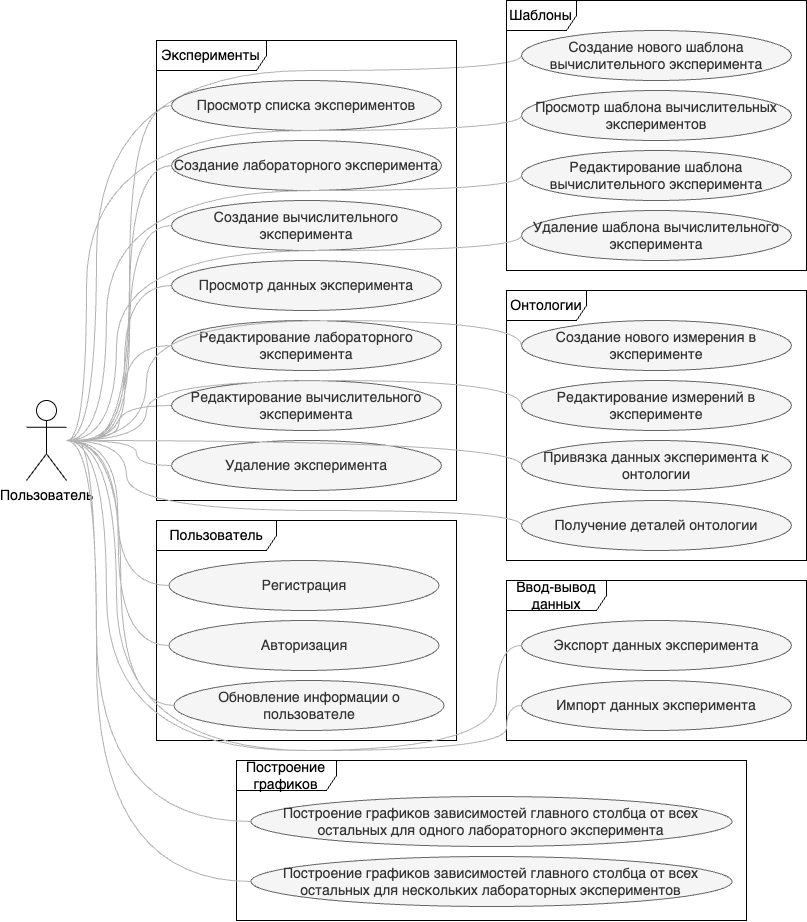
\includegraphics[width=0.35\linewidth]{img/use_cases.png}
    \caption{Диаграмма пользовательских сценариев}
    \label{pic:uc}
\end{figure}

\subsection{Архитектура приложения}

\subsubsection{Схема базы данных}

Таблица \texttt{users} хранит информацию о пользователях системы.
Поле \texttt{id} является уникальным идентификатором пользователя. Поле \texttt{username} содержит уникальный логин пользователя, поле \texttt{hashed\_password} используется для хранения зашифрованного пароля.

Таблица \texttt{profiles} расширяет информацию о пользователе, включая имя, фамилию и дату регистрации.
Поле \texttt{user\_id} ссылается на таблицу \texttt{users}, обеспечивая связь с учётной записью пользователя.

Таблица \texttt{experiments} хранит данные, общие для всех типов экспериментов.
Поле \texttt{id} -- уникальный идентификатор эксперимента, поле \texttt{path} хранит полный путь до эксперимента, поле \texttt{description} -- его описание, поле \texttt{kind} -- вид эксперимента (лабораторный или вычислительный). Поле \texttt{user\_id} ссылается на пользователя, создавшего эксперимент. Поля \texttt{created\_at} и \texttt{updated\_at} фиксируют дату и время создания и последнего редактирования эксперимента соответственно.

Таблица \texttt{lab\_experiments} хранит данные о лабораторных экспериментах.
Поле \texttt{id} -- уникальный идентификатор эксперимента, является внешним ключом на поле \texttt{experi-\allowbreak ments.id}, таким образом образуя уникальное подмножество значений этого поля.
Также является точкой расширения информации о лабораторных экспериментах в будущем.

Таблица \texttt{columns} хранит информацию о столбцах таблиц измерений в лабораторных экспериментах.
Поле \texttt{id} -- уникальный идентификатор столбца, поле \texttt{name} -- имя столбца, поле \texttt{ontology} -- псевдоним онтологии (онтология должна быть зарегистрирована в приложении под этим псевдонимом), поле \texttt{ontology\_ref} содержит URI элемента из онтологии, указанной в поле \texttt{ontology}, поле \texttt{is\_main} указывает, является ли столбец главной (исследуемой) переменной, это нужно для построения графиков зависимостей.

Таблица \texttt{measurements} используется для хранения данных в лабораторных экспериментах в узком формате, то есть тройками вида \texttt{(row, column, value)}.
Поле \texttt{id} является уникальным идентификатором записи.
Поле \texttt{experiment\_id} ссылается на эксперимент из таблицы \texttt{lab\_experiments}.

Таблица \texttt{schemas} хранит схемы данных для вычислительных экспериментов.
Поле \texttt{id} -- уникальный идентификатор схемы.
Поле \texttt{type} хранит одно из значений множества \texttt{{INPUT, OUTPUT, PARAMETERS, CONTEXT}}.
Поле \texttt{data} описывает сами данные в формате JSONB.

Таблица \texttt{computational\_templates} хранит шаблоны для вычислительных экспериментов.
Поле \texttt{id} -- уникальный идентификатор шаблона. Поле \texttt{path} -- полный путь до шаблона, поля \texttt{input\_id}, \texttt{output\_id}, \texttt{parameters\_id}, \texttt{context\_id} ссылаются на поле \texttt{schemas.id}, означая соответственно ссылки на схемы входных и выходных данных, параметров эксперимента, а также контекста -- дополнительных данных, которые могут быть использованы в эксперименте, но не привязаны к онтологиям.

Таблица \texttt{computational\_experiments} хранит вычислительные эксперименты.
Поле \texttt{id} -- уникальный идентификатор эксперимента, является внешним ключом на поле \texttt{experiments.id}, таким образом образуя уникальное подмножество значений этого поля.
Поле \texttt{template\_id} ссылается на поле \texttt{computational\_templates.id}, что означает, что запуски (строки таблицы в пользовательском интерфейсе) эксперимента должны удовлетворять указанному шаблону.

Таблица \texttt{computational\_experiment\_data} хранит данные для вычислительных экспериментов.
Поле \texttt{id} -- уникальный идентификатор запуска эксперимента.
Поле \texttt{experi-\allowbreak ment\_id} ссылается на поле таблицы \texttt{computational\_experiments.id}.
Поля \texttt{input\_id}, \texttt{output\_id}, \texttt{parameters\_id}, \texttt{context\_id} ссылаются на поле \texttt{schemas.id}, означая соответственно ссылки на фактические входные и выходнее данные, параметры и контекст запуска эксперимента.


Общая схема базы данных представлена на рис.~\ref{pic:db}.

\begin{figure}[H]
    \centering
    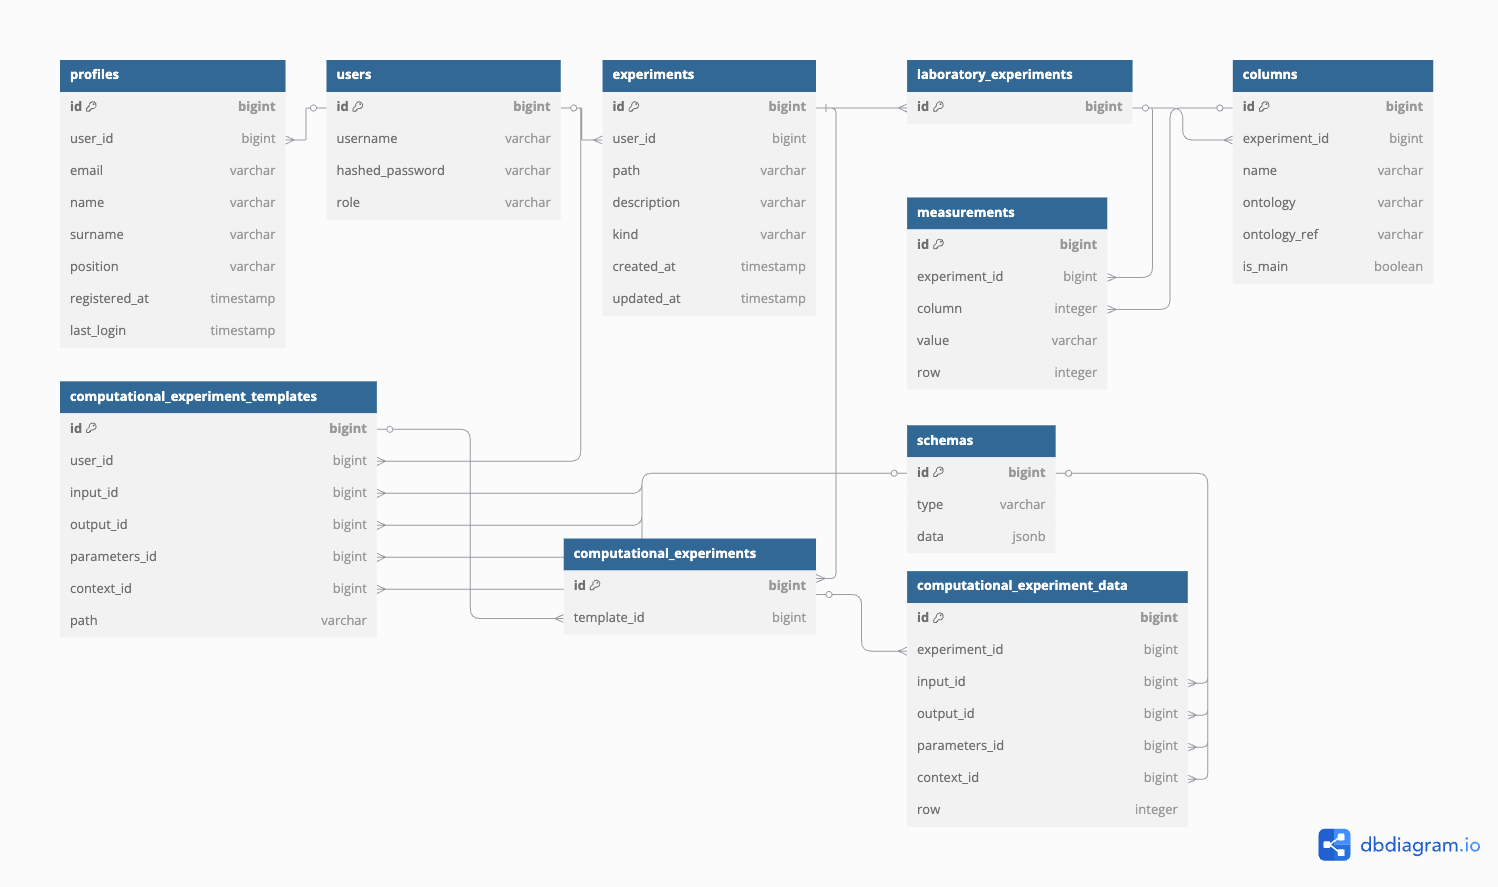
\includegraphics[width=\linewidth]{VKR/img/database_scheme.png}
    \caption{Схема базы данных}
    \label{pic:db}
\end{figure}

\subsubsection{Архитектура серверного приложения}

Выбранная архитектура приложения изображена на рис.~\ref{pic:server_arch} и основана на слоистом подходе, который обеспечивает разделение ответственности между компонентами, улучшает модульность и делает систему более поддерживаемой и масштабируемой.
В серверной части реализована организация слоев: API Router обрабатывает входящие HTTP-запросы и передает их в слой бизнес-логики, где осуществляется основная обработка данных.
Для работы с базами данных используется слой доступа к данным, который взаимодействует с PostgreSQL и Neo4j.
Дополнительно выделены сервис аутентификации и уровень валидации, что обеспечивает безопасность и корректность данных.

\begin{figure}[H]
    \centering
    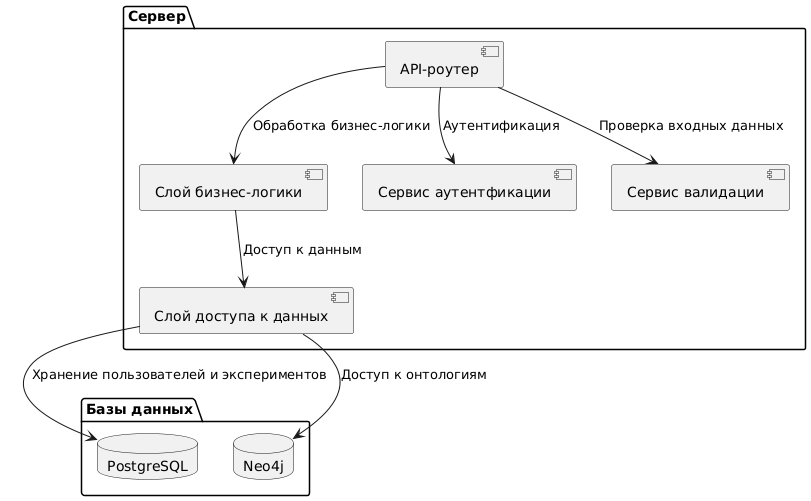
\includegraphics[width=0.7\linewidth]{VKR/img/server_arch.png}
    \caption{Архитектура серверного приложения}
    \label{pic:server_arch}
\end{figure}

\subsubsection{Архитектура клиентского приложения}

Клиентская часть построена на Vue.js и также следует принципам разделения ответственности.
Компоненты пользовательского интерфейса взаимодействуют с хранилищем состояния (Pinia\cite{Library:Pinia}), которое управляет данными и их синхронизацией.
Взаимодействие с сервером осуществляется через API Service, что позволяет отделить сетевые запросы от логики компонентов, а Vue Router\cite{Library:VueRouter} управляет навигацией.
Такой подход обеспечивает гибкость и удобство в разработке.
Архитектура клиентской части изображена на рис.~\ref{pic:client_arch}.

\begin{figure}[H]
    \centering
    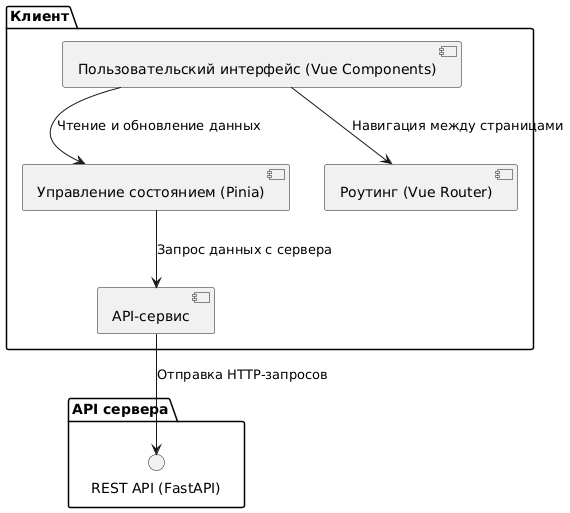
\includegraphics[width=\linewidth]{VKR/img/client_arch.png}
    \caption{Архитектура клиентского приложения}
    \label{pic:client_arch}
\end{figure}

\subsection{Выбор методов и средств реализации}

При выборе технологий для разработки веб-приложения учитывались следующие ключевые требования:
\begin{enumerate}
    \item Производительность и масштабируемость.
    \item Простота интеграции с онтологиями.
    \item Поддержка современных стандартов веб-разработки.
    \item Лёгкость развертывания и сопровождения.
\end{enumerate}

На основании этих критериев были выбраны следующие технологии:

\subsubsection{Выбор фреймворка для серверной части}

В качестве веб-фреймворка для бэкенда было выбрано FastAPI по следующим причинам:
\begin{enumerate}
    \item Высокая производительность -- благодаря использованию Starlette~\cite{Framework:Starlette} и Pydantic~\cite{Library:Pydantic}, FastAPI демонстрирует скорость работы, сопоставимую с Node.js~\cite{Lang:NodeJS} и Go~\cite{Lang:Go}, что особенно важно при работе с API для экспериментов.
    \item Асинхронная обработка запросов -- поддержка async/await позволяет обрабатывать несколько запросов одновременно без блокировки потока выполнения, что критично при обработке вычислительных экспериментов.
    \item Встроенная валидация данных -- благодаря Pydantic, валидация данных выполняется на уровне схем API, уменьшая вероятность ошибок на клиенте и сервере.
    \item Гибкость в интеграции -- поддержка OpenAPI и облегчает документирование и подключение к клиентской части.
\end{enumerate}

Альтернативными вариантами были Django Rest Framework (DRF)~\cite{Framework:DRF} и Flask~\cite{Framework:Flask}, однако:
\begin{enumerate}
    \item DRF навязывают конкретную архитектуру приложения и имеет ограниченную поддержку асинхронности по сравнению с FastAPI, что противоречит требованию о производительности.
    \item Flask не поддерживает асинхронную обработку "из коробки", что снижает его эффективность для API с высокой нагрузкой.
\end{enumerate}

\subsubsection{Выбор фреймворка для клиентской части}

Для реализации фронтенда был выбран фреймворк Vue.js (Composition API) вместо React~\cite{Framework:React} и Angular~\cite{Framework:Angular}.
Основные причины такого выбора:
\begin{enumerate}
    \item Лёгкость освоения и высокая продуктивность -- Vue.js имеет интуитивно понятный синтаксис и гибкость в использовании как декларативного программирования, так и компонентов.
    \item Композиционный API -- использование Composition API в Vue 3 улучшает переиспользуемость кода и упрощает управление состоянием.
    \item Высокая производительность -- виртуальный DOM оптимизирован, механизм реактивности позволяет минимизировать ререндеринг.
    \item Гибкость в архитектуре -- Vue.js легко интегрируется с серверными приложениями через REST API.
\end{enumerate}

В качестве альтернатив рассматривались:
\begin{enumerate}
    \item React -- мощный, но требует дополнительной конфигурации и использования сторонних библиотек для маршрутизации и управления состоянием.
    \item Angular -- мощный, но имеет высокие накладные расходы на разработку.
\end{enumerate}

\subsubsection{Выбор библиотеки для пользовательского интерфейса}

Библиотека компонентов PrimeVue~\cite{Framework:PrimeVue} выбрана для реализации интерфейса по следующим причинам:
\begin{enumerate}
    \item Готовые UI-компоненты -- ускоряют разработку благодаря наличию таблиц, форм, модальных окон и других элементов.
    \item Поддержка тем -- пакет предоставляет несколько готовых тем, позволяющих легко менять визуальное оформление.
    \item Гибкость -- компоненты адаптируются под мобильные и десктопные устройства.
\end{enumerate}

Альтернативой был Vuetify~\cite{Framework:Vuetify}, но в нём отсутствуют некоторые необходимые компоненты (например, дерево элементов, полезное для отображения экспериментов и шаблонов), также он навязывает подход Material Design~\cite{Framework:MaterialDesign}.
Ещё более значительным минусом Vuetify является больший по сравнению с другими библиотеками~\cite{Proofs:CompareUILibraries} размер итогового бандла – файла, в который упакован весь необходимый код, отправляемый браузеру.

\subsubsection{Выбор реляционной СУБД}

В качестве основной базы данных была выбрана PostgreSQL, поскольку:
\begin{enumerate}
    \item Поддерживает сложные реляционные структуры -- идеально подходит для хранения экспериментов, пользователей и привязок к онтологиям.
    \item Расширенные возможности JSONB -- позволяет эффективно хранить и обрабатывать JSON-документы без использования NoSQL-решений.
    \item Высокая производительность -- оптимизированные индексы и транзакции позволяют обрабатывать большие объёмы данных.
\end{enumerate}

Наиболее конкурентоспособная альтернатива – MySQL~\cite{DB:MySQL}, но данная СУБД медленнее работает с JSON в режиме чтения~\cite{Proofs:Postgres-vs-MySQL}, что важно для нашего приложения, так как эксперимент просматривается чаще, чем редактируется.

\subsubsection{Выбор графовой СУБД}

Так как приложение активно работает с онтологиями, было принято решение использовать Neo4j для хранения и обработки онтологических связей:
\begin{enumerate}
    \item Графовая структура -- идеально подходит для представления онтологий, где между сущностями существует множество взаимосвязей.
    \item Cypher Query Language~\cite{QueryLang:CypherQL} -- позволяет легко выполнять сложные запросы, например, нахождение зависимостей между измерениями.
    \item Гибкость -- позволяет расширять базу знаний без нарушения структуры данных.
    \item Плагин neosemantics~\cite{Library:NeoSemantics} – позволяет удобно работать с онтологиями, представленными в RDF/XML.
\end{enumerate}

\subsubsection{Выбор средств развёртывания}

Для контейнеризации приложения используется Docker Compose~\cite{Tool:DockerCompose}, по следующим причинам:
\begin{enumerate}
    \item Простота конфигурации -- управление контейнерами через docker-compose.yml не требует сложных манифестов.
    \item Более удобен для разработки -- локальная среда легко воспроизводится на разных машинах.
    \item Не требует дополнительного оркестратора -- Kubernetes~\cite{Tool:Kubernetes} сложен в настройке и требует значительных ресурсов.
    \item Быстрое развертывание -- приложение запускается одной командой, обеспечивая автоматический запуск всех сервисов.
\end{enumerate}

Kubernetes рассматривался как альтернатива, но его сложность оправдана только для высоконагруженных распределённых систем, что не является текущей целью проекта.

\anonsubsection{Выводы по главе}

В результате проектирования были сформированы пользовательские сценарии, отражающие ключевые действия исследователя в системе, включая работу с лабораторными и вычислительными экспериментами, онтологиями, а также процесс регистрации, авторизации и экспорта данных.
Эти сценарии легли в основу проектных решений, обеспечивающих удобство интерфейса.

Разработанная архитектура приложения охватывает как клиентскую, так и серверную части, обеспечивая разделение ответственности, масштабируемость и расширяемость.
Использование современных технологий, таких как FastAPI, PostgreSQL, Vue.js и Neo4j, позволило заложить основу для эффективного взаимодействия между компонентами системы и гибкого управления экспериментальными данными.

Сформированная схема базы данных обеспечивает хранение всех ключевых сущностей предметной области: пользователей, экспериментов, измерений, онтологий и шаблонов.
Она поддерживает как лабораторные, так и вычислительные эксперименты, а также обеспечивает необходимую связность между всеми элементами.

Таким образом, результаты проектирования представляют собой завершённую и целостную концепцию системы, обеспечивающую все предусмотренные функциональные и архитектурные требования, и готовую к этапу реализации.